\documentclass[onlytextwidth]{beamer}
\documentclass[onlytextwidth]{beamer}
\usepackage[utf8]{inputenc}
\usepackage{microtype}
\usepackage{amsmath}
\usepackage{amssymb}
\usepackage[nomessages]{fp} %\FPeval{\var-name}{2*sin(pi/6)}
\usepackage{siunitx} %units in math. eg 20\milli\meter
\usepackage{yhmath} % for arcs, overparenth command
\usepackage{tikz} %graphics
\usetikzlibrary{quotes, angles}
%\usepackage{graphicx} already loaded by beamer class
%consider setting \graphicspath{{images/}}
%\parskip ?? to avoid paragraph indent
\usepackage{multicol} %may not need this package, just columns environment
\usepackage{venndiagram}

\subtitle[BECA]{Bronx Early College Academy}
\author[Huson]{Christopher J. Huson PhD}

\setbeamertemplate{headline}{\vskip2mm 
  BECA / \insertshortauthor \, / \inserttitle
  \hfill 
  \insertsection
  }

\title{Modeling and Mathematics Applications}
\date{2023-2024}

\begin{document}
\frame{\titlepage}

%\section[Outline]{}
%\frame{\tableofcontents}

\section{Course description \hfill 13 November}
\begin{frame}{A course for students \emph{interested} in mathematics}
  \begin{block}{A modern approach to teaching and learning}
  \begin{enumerate}
      \item Important topics in mathematics skipped in regular classes
      \item ``Modeling'' is a method to solve practical problems
      \item Also include important proofs in theoretical mathematics \\
      (primes are infinite, $\sqrt{2}$ is irrational, there are different sizes of infinity)
      \item Collaborative, small group, discourse oriented
      \item Project-based assessments
  \end{enumerate}
  \end{block}
  \end{frame}

\begin{frame}{Class schedule prepares you for college and career}
  {Official course on your transcript, $\frac{1}{2}$ credit}
  \begin{block}{In-person instruction}
    \begin{enumerate}
      \item Monday \& Tuesday: 1:24 - 2:20
      \item Lunch will be brought up from the cafeteria
    \end{enumerate}
    \end{block}
  \begin{block}{Online coursework}
    \begin{enumerate}
      \item One hour on Saturdays at a time to be determined
      \item Small groups working independently
    \end{enumerate}
    \end{block}
    \begin{block}{Google Classroom}
      \begin{enumerate}
        \item Official course materials and assignments
        \item Also \href{https://math.huson.com}{math.huson.com} and GitHub
      \end{enumerate}
      \end{block}
  \end{frame}

\begin{frame}{Take class notes in a composition book}
  \begin{block}{Use this notebook format (required)}
    \begin{enumerate}
      \item Outside cover: ``Modeling'' or ``Applied Math'', your first and last name
      \item First page: your name, my contact info \\
      \qquad Dr. Huson / chuson@schools.nyc.gov / 917-648-5632 \vspace{0.25cm}
      \item Your passwords and logins
    \end{enumerate}
    \end{block}
  \end{frame}
    
\begin{frame}{Computers in mathematics}
  \begin{block}{A new way of learning mathematics in school}
    \begin{enumerate}
      \item Machines for calculation and formatting \\
      People for understanding, communicating, questioning
      \item Changing the types of problems we try to solve \\[0.25cm]
      Warning:
      \item Programming is time consuming and frustrating
      \item Real world tools require your attention to privacy and security
    \end{enumerate}
    \end{block}
    \begin{block}{Artificial intelligence is a threat and an opportunity (for you)}
      \begin{enumerate}
        \item Microsoft / OpenAI tools: ChatGPT-4, Bing/Edge, Copilot
        \item Logical thinking and articulation are even more important
      \end{enumerate}
      \end{block}
  \end{frame}

\section{A new perspective on mathematics}
\begin{frame}{Change your view of what it means to be able to \emph{do} mathematics}
      \begin{columns}[T]
        \begin{column}{0.5\textwidth}
          \begin{block}{}\vspace{0.5cm}
            ``In the middle of every difficulty lies opportunity.'' \\[0.5cm]
            ``Do not worry about your difficulties in mathematics, I assure you that mine are greater.'' \\[0.5cm]
            \href{https://yourstory.com/2023/04/embrace-adversity-unlock-opportunities}{Albert Einstein}
          \end{block}
        \end{column}
        \begin{column}{0.5\textwidth}
          \begin{figure}
            \centering
            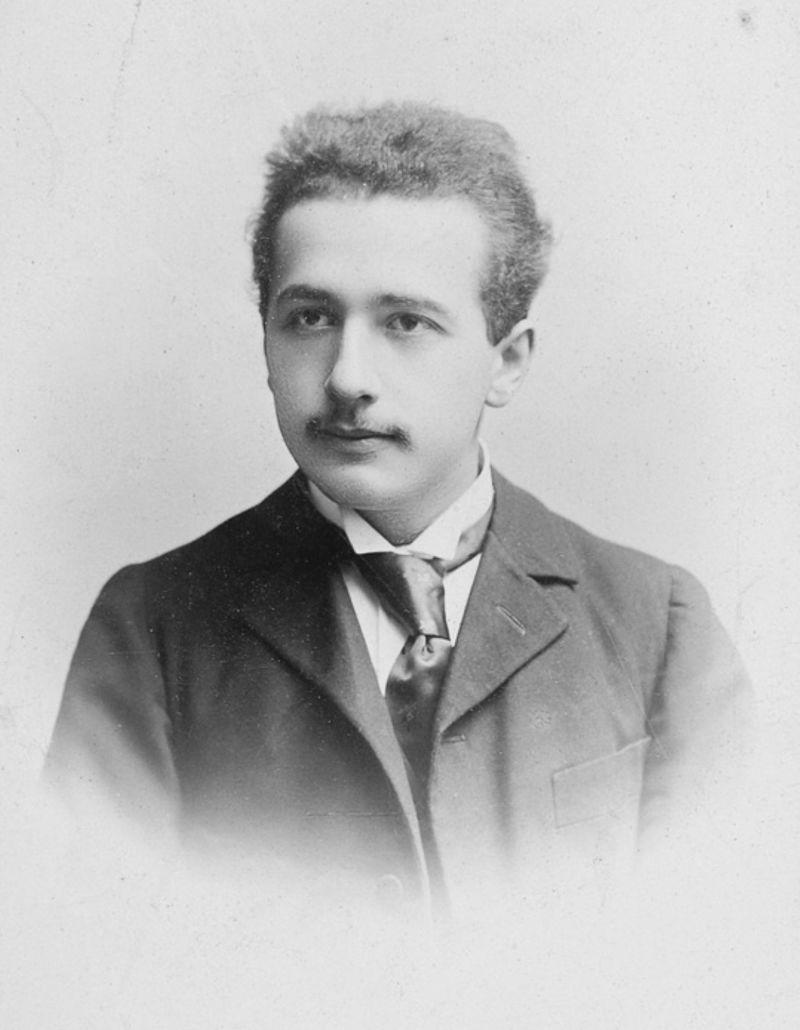
\includegraphics[width=0.8\textwidth]{../graphics/Albert_Einstein_c1890s.jpg}
            \caption{Albert Einstein c1890s}
          \end{figure}
        \end{column}
      \end{columns}
    \end{frame}

  

\end{document}
Follow with Einstein quote about posing problems